\documentclass[11pt]{article}
\usepackage[utf8]{inputenc}
\usepackage[T1]{fontenc}
\usepackage{amsmath}
\usepackage{amssymb}
\usepackage{multicol}
\usepackage{geometry}
\usepackage{tikz}
\usepackage{enumitem}
\usepackage{xcolor}
\usepackage{titlesec}

% Configurações de layout
\geometry{a4paper, left=1cm, right=1cm, top=0.5cm, bottom=1.2cm}
\setlength{\columnseprule}{0.4pt}

% Cores para títulos
\titleformat{\section}{\normalfont\Large\bfseries\color{blue}}{\thesection}{1em}{}
\titleformat{\subsection}{\normalfont\large\bfseries\color{red}}{\thesubsection}{1em}{}

\title{\textcolor{red}{Segundo Trimestre: Matemática Financeira
    \\Juros Simples e Compostos}}
\author{Professor: Jefferson}
\date{}

\begin{document}

\maketitle
\vspace{-1cm}

%\begin{center}
%\large{Nome: \underline{\hspace{8cm}} \quad Turma: \underline{\hspace{3cm}}}
%\end{center}

\begin{multicols}{2}

\section*{Conceitos Básicos}

\subsection*{Capital (C)}
Valor inicial aplicado ou emprestado.

\subsection*{Taxa de Juros (i)}
Porcentagem cobrada pelo empréstimo ou ganha pelo investimento.

\subsection*{Tempo (t)}
Período da aplicação (em meses, anos, etc.).

\subsection*{Montante (M)}
Valor total ao final do período:
\[
M = C + J
\]
onde $J$ são os juros.

\section*{Juros Simples}

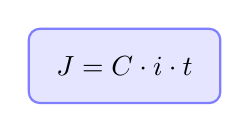
\begin{tikzpicture}
\node[rectangle, fill=blue!10, rounded corners, inner sep=10pt, draw=blue!50, thick] (box) {
$\displaystyle J = C \cdot i \cdot t$
};
\end{tikzpicture}

\textbf{Fórmulas:}
\begin{itemize}
\item Juros: $J = C \cdot i \cdot t$
\item Montante: $M = C \cdot (1 + i \cdot t)$
\item Capital: $C = \dfrac{M}{1 + i \cdot t}$
\item Taxa: $i = \dfrac{J}{C \cdot t}$
\item Tempo: $t = \dfrac{J}{C \cdot i}$
\end{itemize}

\textbf{Características:}
\begin{itemize}
\item Juros constantes por período
\item Crescimento linear
\item Calculado sempre sobre o capital inicial
\end{itemize}

\section*{Juros Compostos}

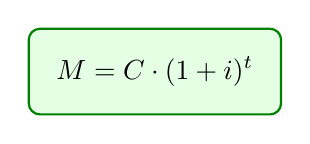
\begin{tikzpicture}
\node[rectangle, fill=green!10, rounded corners, inner sep=10pt, draw=green!50!black, thick] (box) {
$\displaystyle M = C \cdot (1 + i)^t$
};
\end{tikzpicture}

\textbf{Fórmulas:}
\begin{itemize}
\item Montante: $M = C \cdot (1 + i)^t$
\item Juros: $J = M - C = C \cdot [(1 + i)^t - 1]$
\item Capital: $C = \dfrac{M}{(1 + i)^t}$
\item Taxa: $i = \sqrt[t]{\dfrac{M}{C}} - 1$
\item Tempo: $t = \dfrac{\log\left(\frac{M}{C}\right)}{\log(1 + i)}$
\end{itemize}

\textbf{Características:}
\begin{itemize}
\item Juros sobre juros (juros capitalizados)
\item Crescimento exponencial
\item Mais usado no mercado financeiro
\end{itemize}

\section*{Comparação}

\begin{center}
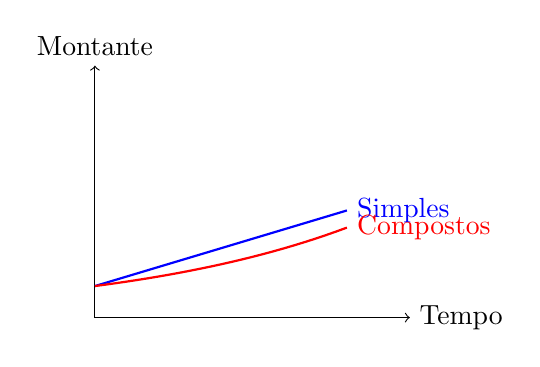
\begin{tikzpicture}[scale=0.8]
\draw[->] (0,0) -- (5,0) node[right] {Tempo};
\draw[->] (0,0) -- (0,4) node[above] {Montante};
\draw[blue, thick, domain=0:4] plot (\x, {0.5 + 0.3*\x}) node[right] {Simples};
\draw[red, thick, domain=0:4] plot (\x, {0.5*(1.3^\x)}) node[right] {Compostos};
\end{tikzpicture}
\end{center}

\textbf{Diferenças:}
\begin{itemize}
\item \textbf{Simples}: Linear, juros fixos por período
\item \textbf{Compostos}: Exponencial, juros sobre juros
\item Para $t > 1$: Compostos sempre rende mais
\end{itemize}

\section*{Exercícios Básicos}

\begin{enumerate}[leftmargin=*]

\item Calcule os juros simples:
\begin{enumerate}[label=\alph*)]
\item $C = R\$ 1000$, $i = 2\%$ a.m., $t = 6$ meses
\item $C = R\$ 500$, $i = 1,5\%$ a.m., $t = 1$ ano
\item $C = R\$ 2000$, $i = 10\%$ a.a., $t = 2$ anos
\end{enumerate}

\item Calcule o montante a juros compostos:
\begin{enumerate}[label=\alph*)]
\item $C = R\$ 1000$, $i = 2\%$ a.m., $t = 6$ meses
\item $C = R\$ 500$, $i = 1,5\%$ a.m., $t = 12$ meses
\item $C = R\$ 2000$, $i = 10\%$ a.a., $t = 2$ anos
\end{enumerate}

\item Compare os dois sistemas para:
\begin{enumerate}[label=\alph*)]
\item $C = R\$ 1000$, $i = 5\%$ a.a., $t = 3$ anos
\item $C = R\$ 5000$, $i = 2\%$ a.m., $t = 8$ meses
\end{enumerate}

\item Resolva os problemas:
\begin{enumerate}[label=\alph*)]
\item João aplicou R\$ 800 a juros simples de 3\% a.m. por 5 meses. Qual o montante?
\item Maria investiu R\$ 1500 a juros compostos de 2\% a.m. por 1 ano. Quanto ela terá?
\end{enumerate}

\item Calcule a taxa mensal equivalente a:
\begin{enumerate}[label=\alph*)]
\item 12\% a.a. (juros simples)
\item 12\% a.a. (juros compostos)
\item 24\% a.a. (juros compostos)
\end{enumerate}

\end{enumerate}

\section*{Exercícios Intermediários}

\begin{enumerate}[leftmargin=*, start=6]

\item Um capital de R\$ 2000 foi aplicado:
\begin{enumerate}[label=\alph*)]
\item A juros simples: rendeu R\$ 600 em 1 ano. Qual a taxa anual?
\item A juros compostos: transformou-se em R\$ 2420 em 1 ano. Qual a taxa anual?
\end{enumerate}

\item Determine o tempo necessário para:
\begin{enumerate}[label=\alph*)]
\item Duplicar um capital a juros simples de 10\% a.a.
\item Duplicar um capital a juros compostos de 10\% a.a.
\item Triplicar um capital a juros compostos de 5\% a.m.
\end{enumerate}

\item Problemas mistos:
\begin{enumerate}[label=\alph*)]
\item Qual é mais vantajoso: 
  R\$ 1000 por 2 anos a 8\% a.a. (simples) ou
  R\$ 1000 por 2 anos a 7,5\% a.a. (compostos)?
\item Um investimento de R\$ 5000 rendeu R\$ 800 em 8 meses. 
  Qual a taxa mensal se foram juros simples?
\end{enumerate}

\item Complete a tabela:
\begin{center}
\begin{tabular}{|c|c|c|c|c|}
\hline
\textbf{C} & \textbf{i} & \textbf{t} & \textbf{J (Simples)} & \textbf{M (Compostos)} \\
\hline
R\$ 1000 & 2\% a.m. & 6 meses & & \\
\hline
R\$ 500 & 12\% a.a. & 2 anos & & \\
\hline
R\$ 2000 & 1,5\% a.m. & 1 ano & & \\
\hline
\end{tabular}
\end{center}

\item Análise de gráficos:
\begin{center}
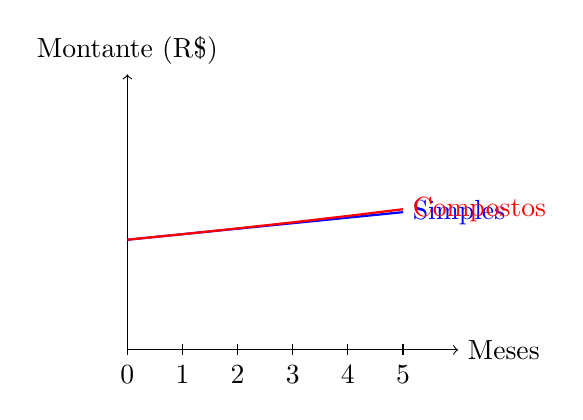
\begin{tikzpicture}[scale=0.7]
\draw[->] (0,0) -- (6,0) node[right] {Meses};
\draw[->] (0,0) -- (0,5) node[above] {Montante (R\$)};
% Juros simples
\draw[blue, thick] (0,2) -- (1,2.1) -- (2,2.2) -- (3,2.3) -- (4,2.4) -- (5,2.5);
% Juros compostos
\draw[red, thick] (0,2) -- (1,2.1) -- (2,2.205) -- (3,2.315) -- (4,2.431) -- (5,2.553);
\node at (5,2.5) [blue, right] {Simples};
\node at (5,2.55) [red, right] {Compostos};
\foreach \x in {0,1,2,3,4,5} \draw (\x,0.1) -- (\x,-0.1) node[below] {\x};
\end{tikzpicture}
\end{center}
\begin{enumerate}[label=\alph*)]
\item Qual o capital inicial?
\item Qual a taxa aproximada?
\item Em que mês a diferença começa a ser significativa?
\end{enumerate}

\end{enumerate}

\section*{Problemas Contextualizados}

\begin{enumerate}[leftmargin=*, start=11]

\item Empréstimo bancário:
\begin{enumerate}[label=\alph*)]
\item Banco A: R\$ 5000, 2\% a.m., 10 meses (simples)
\item Banco B: R\$ 5000, 1,8\% a.m., 10 meses (compostos)
\item Qual é mais vantajoso?
\end{enumerate}

\item Poupança:
\begin{enumerate}[label=\alph*)]
\item Deposito inicial: R\$ 1000
\item Taxa: 0,5\% a.m. (juros compostos)
\item Depósitos mensais: R\$ 200
\item Quanto terá após 1 ano?
\end{enumerate}

\item Financiamento:
\begin{enumerate}[label=\alph*)]
\item Casa: R\$ 150.000
\item Entrada: R\$ 30.000
\item Saldo: R\$ 120.000 em 240 meses a 0,8\% a.m.
\item Qual o valor total pago?
\end{enumerate}

\item Investimento comparativo:
\begin{enumerate}[label=\alph*)]
\item Opção 1: CDB a 12\% a.a. (compostos)
\item Opção 2: Tesouro Direto a 11,5\% a.a. (compostos)
\item R\$ 10.000 por 3 anos
\item Qual rende mais?
\end{enumerate}

\item Juros sobre cheque especial:
\begin{enumerate}[label=\alph*)]
\item Débito: R\$ 800
\item Taxa: 12\% a.m. (compostos)
\item 15 dias de atraso
\item Qual o valor da dívida?
\end{enumerate}

\end{enumerate}

\section*{Exercícios Avançados}

\begin{enumerate}[leftmargin=*, start=16]

\item Taxas equivalentes:
\begin{enumerate}[label=\alph*)]
\item Qual a taxa anual equivalente a 2\% a.m. (compostos)?
\item Qual a taxa mensal equivalente a 26,82\% a.a.?
\item Prove que: $(1 + i_a) = (1 + i_m)^{12}$
\end{enumerate}

\item Tempo de aplicação:
\begin{enumerate}[label=\alph*)]
\item Quanto tempo para R\$ 1000 virar R\$ 2000 a 5\% a.m.?
\item Se R\$ 5000 rendeu R\$ 1000 em 4 meses, qual a taxa mensal (compostos)?
\end{enumerate}

\item Problema de lógica:
\begin{enumerate}[label=\alph*)]
\item Um capital aplicado a juros simples duplica em 10 anos.
  Em quanto tempo triplicaria?
\item Um capital aplicado a juros compostos triplica em 5 anos.
  Em quanto tempo quadruplicaria?
\end{enumerate}

\item Análise de investimento:
\begin{enumerate}[label=\alph*)]
\item Projeto A: Retorno de 15\% a.a. em 3 anos
\item Projeto B: Retorno de 12\% a.a. em 5 anos
\item R\$ 50.000 disponíveis
\item Qual projeto escolher?
\end{enumerate}

\item Desafio:
\begin{enumerate}[label=\alph*)]
\item Um banco oferece: "Duplique seu dinheiro em 5 anos!"
  Qual a taxa anual de juros compostos?
\item Verifique se é melhor: 1\% a.m. ou 12,68\% a.a.
\end{enumerate}

\end{enumerate}

\section*{Fórmulas Importantes}

\subsection*{Conversão de Taxas}

\textbf{Juros Simples:}
\[
i_{\text{anual}} = 12 \cdot i_{\text{mensal}}
\]

\textbf{Juros Compostos:}
\[
1 + i_a = (1 + i_m)^{12}
\]
\[
i_m = \sqrt[12]{1 + i_a} - 1
\]

\subsection*{Regras Práticas}

\begin{itemize}
\item \textbf{Regra do 72}: Para estimar tempo de duplicação:
  \[
  t \approx \frac{72}{i(\%)}
  \]
\item \textbf{Diferença aumenta} com o tempo
\item \textbf{Prazos curtos}: Diferença pequena
\item \textbf{Prazos longos}: Compostos muito superiores
\end{itemize}

\section*{Dicas para Resolver}

\begin{itemize}
\item \textbf{Identifique}: Simples ou composto?
\item \textbf{Unidades}: Taxa e tempo na mesma unidade
\item \textbf{Cuidado}: 1 ano = 12 meses (não 10!)
\item \textbf{Verifique}: Resposta faz sentido?
\item \textbf{Compare}: Sempre calcule os dois para entender diferenças
\item \textbf{Use calculadora}: Para potências e logaritmos
\end{itemize}

\section*{Aplicações Práticas}

\begin{itemize}
\item \textbf{Poupança}: Juros compostos
\item \textbf{Cheque especial}: Juros compostos altos
\item \textbf{Financiamentos}: Juros compostos
\item \textbf{Investimentos}: Compare taxas equivalentes
\item \textbf{Empréstimos}: Atenção aos juros!
\end{itemize}

\end{multicols}

\end{document}
